\section{Performance Testing}

We have performed a lot of testing in the software realm and have had a minimally viable product in the simulator for months now. We've run the simulator in various environmental setups, from a few to many lanes, with differing gaps and with different layouts and densities of obstacles. We are pretty confident in our performance in this setting. There is noise in the simulated sensor data and controls, but we know the simulator performance is still an idealized view of our performance potential.

We frequently do drive checks in our lab and in the adjacent hallways to verify functionality as we make changes. We've done a few large-scale tests on a grassy field on which we could paint white lanes using grass chalk spray. These test days gave us insight into flawed areas that we needed to focus on with mechanical and electrical aspects. We used these days to record tons of camera data to train the CNN and simulate the competition with more realistic camera inputs than the simulator provides. 

\begin{figure}[h]
    \centering
    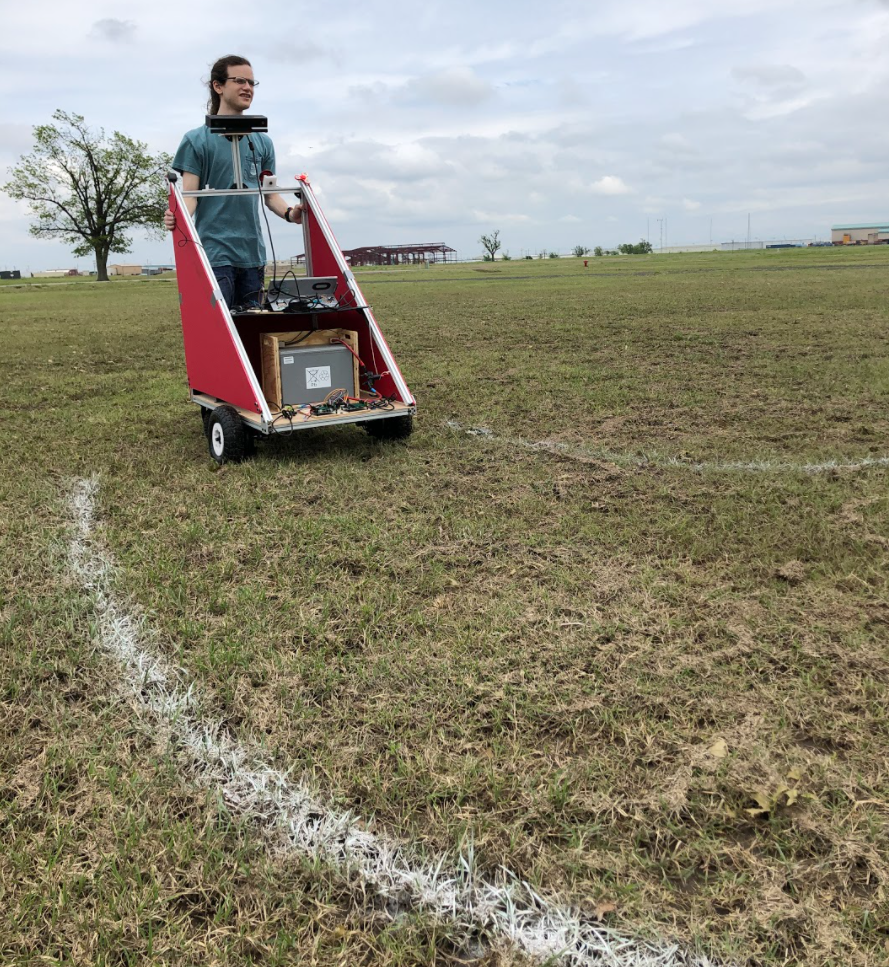
\includegraphics[width=0.4\textwidth]{images/outdoor_test.PNG}
    \caption{Outdoor test of our robot in a painted grassy field.}
\end{figure}

This testing was done before the announcement that this year's competition would take place on asphalt rather than grass, which forced us to make adjustments to both the robot design and our plans for further testing. We were still able to use the data we gathered by tinting all grass in the images to a dark grey to approximate a parking lot, but we aren't able to get free access to a real parking lot to cover lanes and paint our own. This means we can't have as much confidence in our lane detection as we could with grass, but in the worst case we will be able to take additional camera footage during the testing days once we arrive to the competition venue, and can feed that through to tune the CNN to the exact conditions we'll see in the competition.

